% !LW recipe=lualatex x2
\documentclass[aspectratio=169,10pt,xcolor=table]{beamer}

% ============================================================
% Official HUST Beamer theme (red, 16:9), vendored in hust-beamer/
% -- see hust-beamer/README.md for its source. Compile with
% LuaLaTeX (twice) so the Lato and TeX Gyre Adventor fonts are found.
% ============================================================
\makeatletter
\def\input@path{{hust-beamer/}}
\makeatother
\usetheme[
  color=red,
  font=lato,
  titlefont=avantgarde,
  footerlogo=full,
  bar=thin,
  titlepage=cover,
  sectionpage=panel,
  numbering=fraction,
  progressbar=on,
  footermeta=on,
  dateaddress=off,
  footerdate={05/11/2026},
  toctitle={Outline},
  reftitle={References}
]{HUST}
\graphicspath{{hust-beamer/assets/}{figures/}}
\usepackage{booktabs}
% The theme draws with these TikZ libraries; its optional hust-setup.tex
% (not used here) would otherwise load them.
\usetikzlibrary{calc, decorations.markings, arrows.meta}
% Wider cover text block, so the subtitle stays on one line
\makeatletter
\hust@param{coverTextW}{0.7000}{0.8030}
\makeatother

% ---- Shared colours and macros ----
\definecolor{cardgray}{HTML}{F2F2F2}
\definecolor{inkgray}{HTML}{55585B}

% Numbered circle used on the preparation cards
\newcommand{\cardbadge}[1]{\tikz[baseline=-0.65ex]{\node[circle, fill=hustcrimson, text=white, font=\bfseries\small, inner sep=0pt, minimum size=20pt] {#1};}}

% Rounded card, top-aligned: \infocard[fill]{width}{height}{content}
\newcommand{\infocard}[4][cardgray]{%
  \begin{tikzpicture}[baseline=(c.north)]
    \node (c) [fill=#1, rounded corners=5pt, inner sep=7pt] {\parbox[t][#3][t]{#2}{\raggedright #4}};
  \end{tikzpicture}%
}

% Rounded card with natural height: \infobox[fill]{width}{content}
\newcommand{\infobox}[3][cardgray]{%
  \begin{tikzpicture}[baseline=(c.north)]
    \node (c) [fill=#1, rounded corners=5pt, inner sep=7pt] {\parbox[t]{#2}{\raggedright #3}};
  \end{tikzpicture}%
}

% Note box with an amber bar on the left: \notebox{width}{content}
\newcommand{\notebox}[2]{%
  \begin{tikzpicture}[baseline=(c.north)]
    \node (c) [fill=hustamber!14, inner sep=7pt] {\parbox[t]{#1}{\raggedright #2}};
    \draw[hustamber, line width=3pt] ([xshift=1.5pt]c.north west) -- ([xshift=1.5pt]c.south west);
  \end{tikzpicture}%
}

% Number tile used on the model evaluation slide
\newcommand{\stattile}[2]{%
  \begin{tikzpicture}
    \node[rounded corners=6pt, fill=cardgray, inner sep=6pt, minimum width=2.9cm, align=center] {%
      \begin{minipage}{2.5cm}\centering
        {\color{hustcrimson}\bfseries\large #1}\\[0pt]
        {\scriptsize\color{inkgray} #2}
      \end{minipage}%
    };
  \end{tikzpicture}%
}

\title[Profit-Driven Discount Strategy]{Profit-Driven Discount Strategy}
\subtitle{Choosing which customers receive a discount to maximise expected profit}
\author[Group 4]{Group 4}
\institute{Business Data Analytics\\Hanoi University of Science and Technology}
\date{05/11/2026}

\begin{document}

\hustsetup{slogantext={}}
\begin{frame}[plain,noframenumbering]
  \titlepage
  \begin{tikzpicture}[remember picture, overlay]
    \node[anchor=north west, align=left, inner sep=0pt, font=\small, text=hustblack]
      at ([xshift=0.0317\paperwidth, yshift=-0.705\paperheight] current page.north west) {%
        \textbf{Instructor:} Nguyễn Bình Minh\\
        \textbf{Group members:}\\
        Nguyễn Bá Anh -- 20261218M\\
        Nguyễn Tiến Khương -- 20261220M\\
        Nguyễn Trọng Huy Hoàng -- 20251191M\\
        Nguyễn Tuệ Lâm -- 20261207M};
  \end{tikzpicture}
\end{frame}

\begin{frame}[noprogressbar]{\husttoctitle}{\husttocsubtitle}
  \tableofcontents[hideallsubsections]
\end{frame}

% One file per part of the talk.
% Business problem: the weekly decision the rest of the talk answers.
\section{Business Problem}

\begin{frame}{Problem statement}{Who should get a retention discount when the weekly budget is fixed?}
  \vspace{0.15cm}
  {\Large Each Monday, the retailer must choose whom to contact within a fixed discount budget.\par}
  \vspace{0.5cm}
  \begin{columns}[T]
    \column{.48\textwidth}
    {\Large\bfseries A purchase we might recover\par}
    \vspace{2pt}
    {\large A customer who would otherwise stop buying may return because of the offer.\par}
    \column{.48\textwidth}
    {\Large\bfseries A purchase we might subsidise\par}
    \vspace{2pt}
    {\large A customer who would buy anyway may use the same discount.\par}
  \end{columns}
  \vspace{0.55cm}
  \begin{block}{Decision criterion}
    \large Maximise expected incremental profit relative to sending no offer.
  \end{block}
\end{frame}

% Data understanding (frames and speaker notes by Lam, ported to the HUST theme).
% Figures: slide/figures/{monthly_revenue_customers,repurchase_gap,rfm_segment_share}.png, taken from
% Lam's final Data Understanding deck (5 Nov 2026);
% numbers: notebooks/01_data_understanding.ipynb and notebooks/02_customer_segments.ipynb.
\section{Data Understanding}

% Gray field card for the data overview: {title}{fields}{use}
\newcommand{\fieldcard}[3]{%
  \infocard{\dimexpr.5\linewidth-17pt\relax}{1.74cm}{%
    {\large\bfseries\color{hustred}#1}\\[1pt]
    {\footnotesize\bfseries #2}\\[1pt]
    {\scriptsize\color{inkgray}#3}}%
}

\begin{frame}{Data overview}{Online Retail II: 1.07M transaction lines from 5,942 customers, Dec 2009 -- Dec 2011}
  \vspace*{-0.27cm}
  \begin{columns}[T]
    \column{.34\textwidth}
    \infocard[hustred]{\dimexpr\linewidth-14pt\relax}{5.15cm}{\color{white}%
      {\scriptsize\bfseries\color{hustsubyellow}DATA SOURCE}\\[1pt]
      {\LARGE\bfseries Online Retail II}\\[2pt]
      {\small Transactions of an online retailer, Dec 2009 -- Dec 2011}\par
      \vspace{0.5cm}
      {\color{hustsubyellow}\rule{\linewidth}{0.8pt}}\par
      \vspace{3pt}
      \begin{tabular}{@{}p{0.58\linewidth}@{}p{0.40\linewidth}@{}}
        {\bfseries\Large 1,067,371} & {\bfseries\Large 53,628}\\[-4pt]
        {\scriptsize transaction lines} & {\scriptsize invoices}\\[2pt]
        {\bfseries\Large 5,942} & {\bfseries\Large \pounds19.3M}\\[-4pt]
        {\scriptsize customers} & {\scriptsize total revenue}\\[2pt]
        {\bfseries\Large 43} & {\bfseries\Large 8}\\[-4pt]
        {\scriptsize countries, UK 91.9\%} & {\scriptsize fields}
      \end{tabular}}
    \column{.64\textwidth}
    \fieldcard{Customer}{Customer ID, Country}{Identify customers and support segmentation.}\hfill
    \fieldcard{Transactions}{Invoice, InvoiceDate, Quantity, Price}{Build order history and purchase metrics.}\par
    \vspace{3pt}
    \fieldcard{Products}{StockCode, Description}{Measure product diversity and purchase patterns.}\hfill
    \fieldcard{Time and labels}{Customer ID, InvoiceDate, valid purchases}{Create observation windows and define churn in the prediction horizon.}\par
    \vspace{3pt}
    \notebox{\dimexpr\linewidth-14pt\relax}{\footnotesize\textbf{Limitation}: no campaign or marketing-cost fields, so campaign ROI cannot be measured directly.}
  \end{columns}
  % Speaker notes (Lam): Our starting question is simple: with a limited retention budget,
  % which customers should we keep, and when should we act? All we have is two years of
  % transactions from an online retailer: about a million lines and 5,900 customers. There
  % are no contracts and no marketing costs, so both value and churn have to be inferred
  % from how people buy. (About 20 seconds)
\end{frame}

\begin{frame}{Revenue and customers}{Revenue is seasonal, and repeat customers carry it}
  \vspace*{-0.15cm}
  \begin{columns}[T]
    \column{.46\textwidth}
    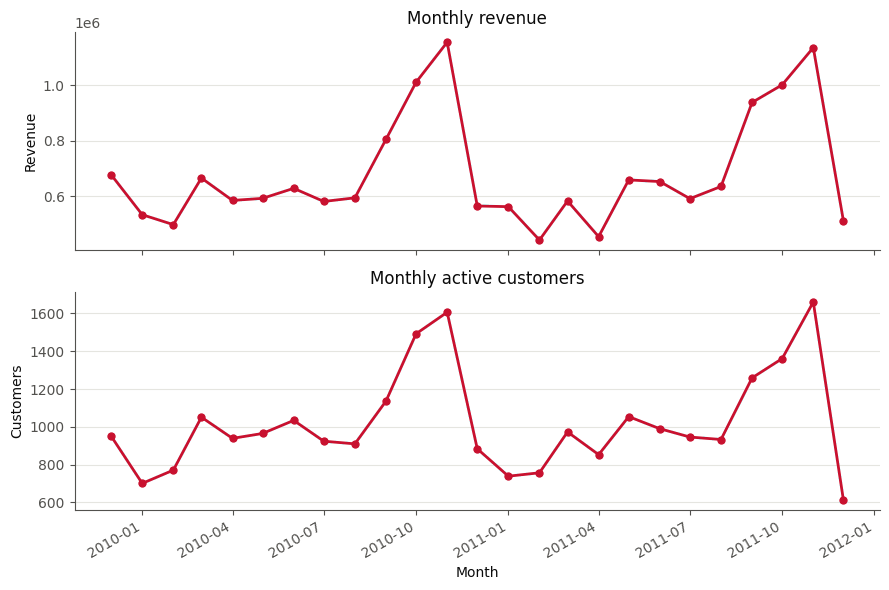
\includegraphics[width=\linewidth]{figures/monthly_revenue_customers.png}
    \column{.52\textwidth}
    \infobox{\dimexpr\linewidth-14pt\relax}{%
      {\large\bfseries\color{hustred}$\sim$1,040 customers/month}\\[3pt]
      {\small\color{inkgray}Median revenue $\approx$ \pounds595K/month (\pounds442K -- \pounds1.16M).}}\par
    \vspace{3pt}
    \notebox{\dimexpr\linewidth-14pt\relax}{%
      {\large\bfseries\color{hustred}Peak in Oct -- Nov}\\[3pt]
      {\small\color{inkgray}Nov 2010: \pounds1.16M $\cdot$ Nov 2011: \pounds1.14M. Pre-Christmas ordering; December drops sharply.}}\par
    \vspace{3pt}
    \infobox[hustred]{\dimexpr\linewidth-14pt\relax}{\color{white}%
      {\large\bfseries 72\% of customers $\rightarrow$ 97\% of revenue}\\[3pt]
      {\small Repeat buyers (72.3\%) generate 95.6\% of orders and 96.7\% of revenue.
      \textcolor{hustsubyellow}{One-time buyers: 27.6\% of customers, 3.3\% of revenue.}}}
  \end{columns}
  % Speaker notes (Lam): Sales are seasonal, peaking before Christmas and dropping sharply
  % in December. More importantly, 72\% of customers buy more than once, and they bring 97\%
  % of revenue. So retention is where the value is. But in retail nobody cancels, so first
  % we need to decide when a customer counts as lost. (About 25 seconds)
\end{frame}

\begin{frame}{Churn definition}{Churn is inferred from purchase rhythm: $H = 90$ days}
  \vspace*{-0.15cm}
  {\small No contracts in retail $\rightarrow$ customers never ``cancel'' $\rightarrow$ churn = no purchase within $H$ days\par}
  \vspace{3pt}
  \begin{columns}[T]
    \column{.45\textwidth}
    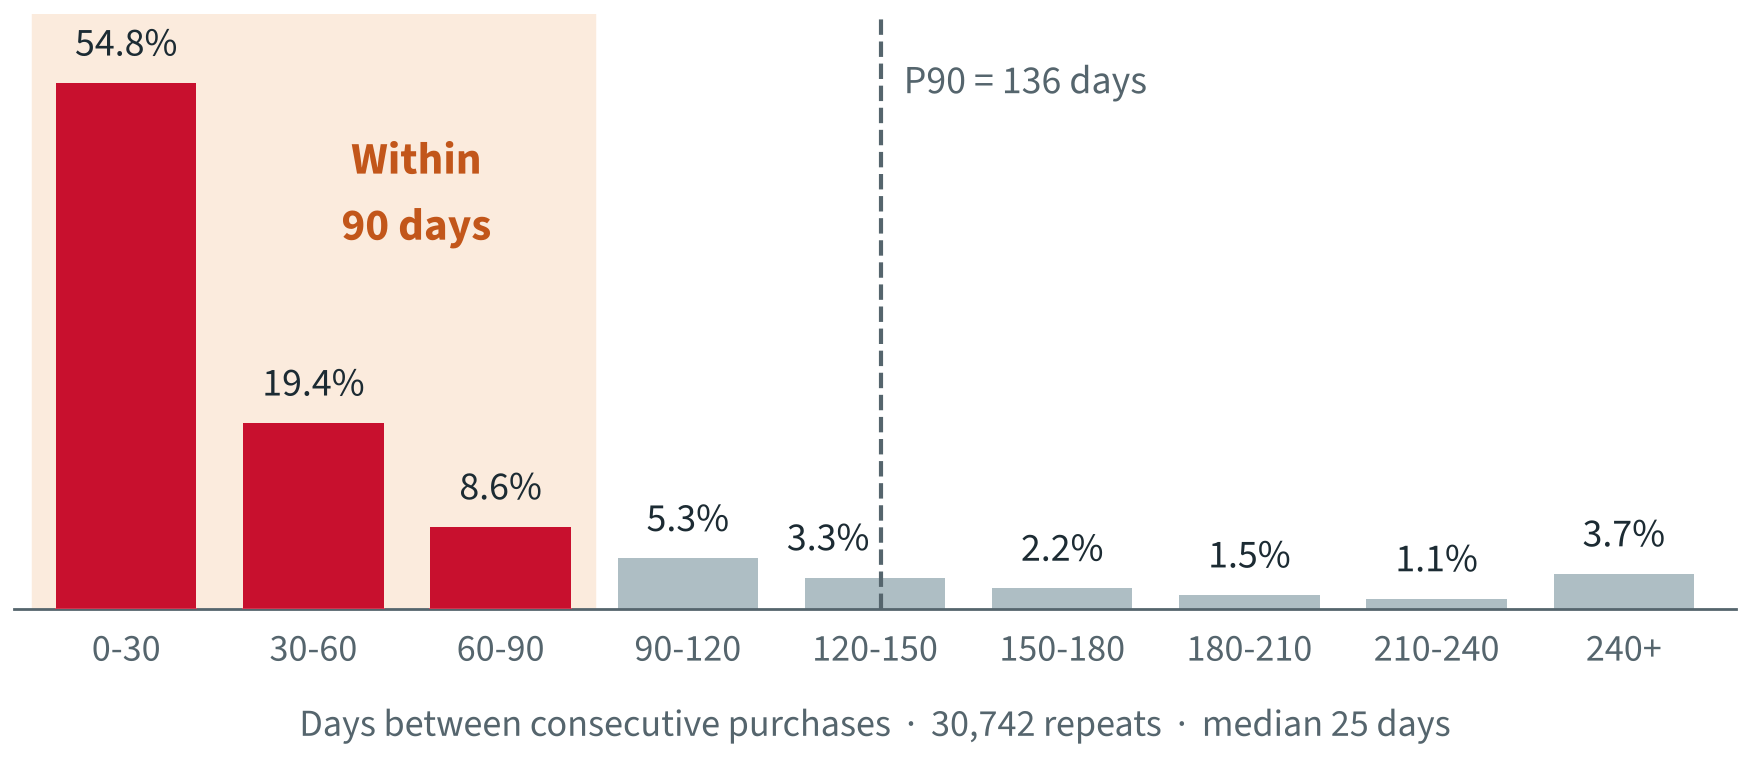
\includegraphics[width=\linewidth]{figures/repurchase_gap.png}
    \column{.52\textwidth}
    \small
    \setlength{\arrayrulewidth}{0.6pt}
    \renewcommand{\arraystretch}{1.15}
    \begin{tabular}{|>{\raggedright\arraybackslash}p{1.35cm}>{\raggedright\arraybackslash}p{2.75cm}>{\raggedright\arraybackslash}p{1.85cm}|}
      \hline
      \rowcolor{hustred}\textcolor{white}{\textbf{$H$}} & \textcolor{white}{\textbf{Repeat purchases within $H$}} & \textcolor{white}{\textbf{Training weeks left}}\\
      \rowcolor{cardgray}60 days & 74.2\% & 37\\
      \bfseries 90 days & \bfseries 82.8\% & \bfseries 24\\
      \rowcolor{cardgray}120 days & 88.1\% & 10\\
      \hline
    \end{tabular}\par
    \vspace{5pt}
    {\small\color{hustred}Short $H$ $\rightarrow$ many false churn labels. Long $H$ $\rightarrow$ late detection, less training data.\par}
  \end{columns}
  \vspace{2pt}
  \infocard{\dimexpr.333\textwidth-18pt\relax}{1.32cm}{%
    {\Large\bfseries\color{hustred}54.8\%}\\[2pt]
    {\scriptsize\color{inkgray}of repeat purchases within 30 days: the largest bin, but not enough}}\hfill
  \infocard{\dimexpr.333\textwidth-18pt\relax}{1.32cm}{%
    {\Large\bfseries\color{hustred}82.8\%}\\[2pt]
    {\scriptsize\color{inkgray}of repeat purchases within 90 days}}\hfill
  \infocard[hustred]{\dimexpr.333\textwidth-18pt\relax}{1.32cm}{\color{white}%
    {\large\bfseries $R_{\max}$ = 136 days (P90)}\\[2pt]
    {\scriptsize No purchase for 136+ days = already gone, nothing left to predict.}}
  % Speaker notes (Lam): We define churn as no purchase within $H$ days, and we set $H$ from
  % the purchase rhythm. More than half of repeat purchases happen within 30 days, but that
  % cutoff would miss too many. At 60 days, one in four repeat purchases would arrive after
  % we had already called the customer churned. At 120 days, we gain only five points but
  % training data drops from 24 weeks to 10. So 90 days is the balance: it covers 83\% of
  % returns. And anyone silent for more than 136 days is effectively gone. (About 35
  % seconds)
\end{frame}

\begin{frame}{Customer segments}{Six behaviour groups; two hold 63\% of revenue}
  \begin{columns}[T]
    \column{.45\textwidth}
    \small
    \renewcommand{\arraystretch}{1.5}
    \begin{tabular}{@{\hspace{6pt}}p{2.75cm}p{3.15cm}@{}}
      \rowcolor{hustred}\textcolor{white}{\textbf{Segment}} & \textcolor{white}{\textbf{Rule}}\\
      \rowcolor{black!20}\textcolor{hustred}{\textbf{Champions}} & Top 10\% M, R $\le$ 90\\
      \rowcolor{black!8}\textcolor{hustred}{\textbf{VIP at risk}} & Top 10\% M, R $>$ 90\\
      \rowcolor{black!20}Loyal & R $\le$ 90, F $\ge$ 4\\
      \rowcolor{black!8}Developing & R $\le$ 90, F = 2--3\\
      \rowcolor{black!20}One-time recent & R $\le$ 90, F = 1\\
      \rowcolor{black!8}Inactive & R $>$ 90
    \end{tabular}
    \column{.53\textwidth}
    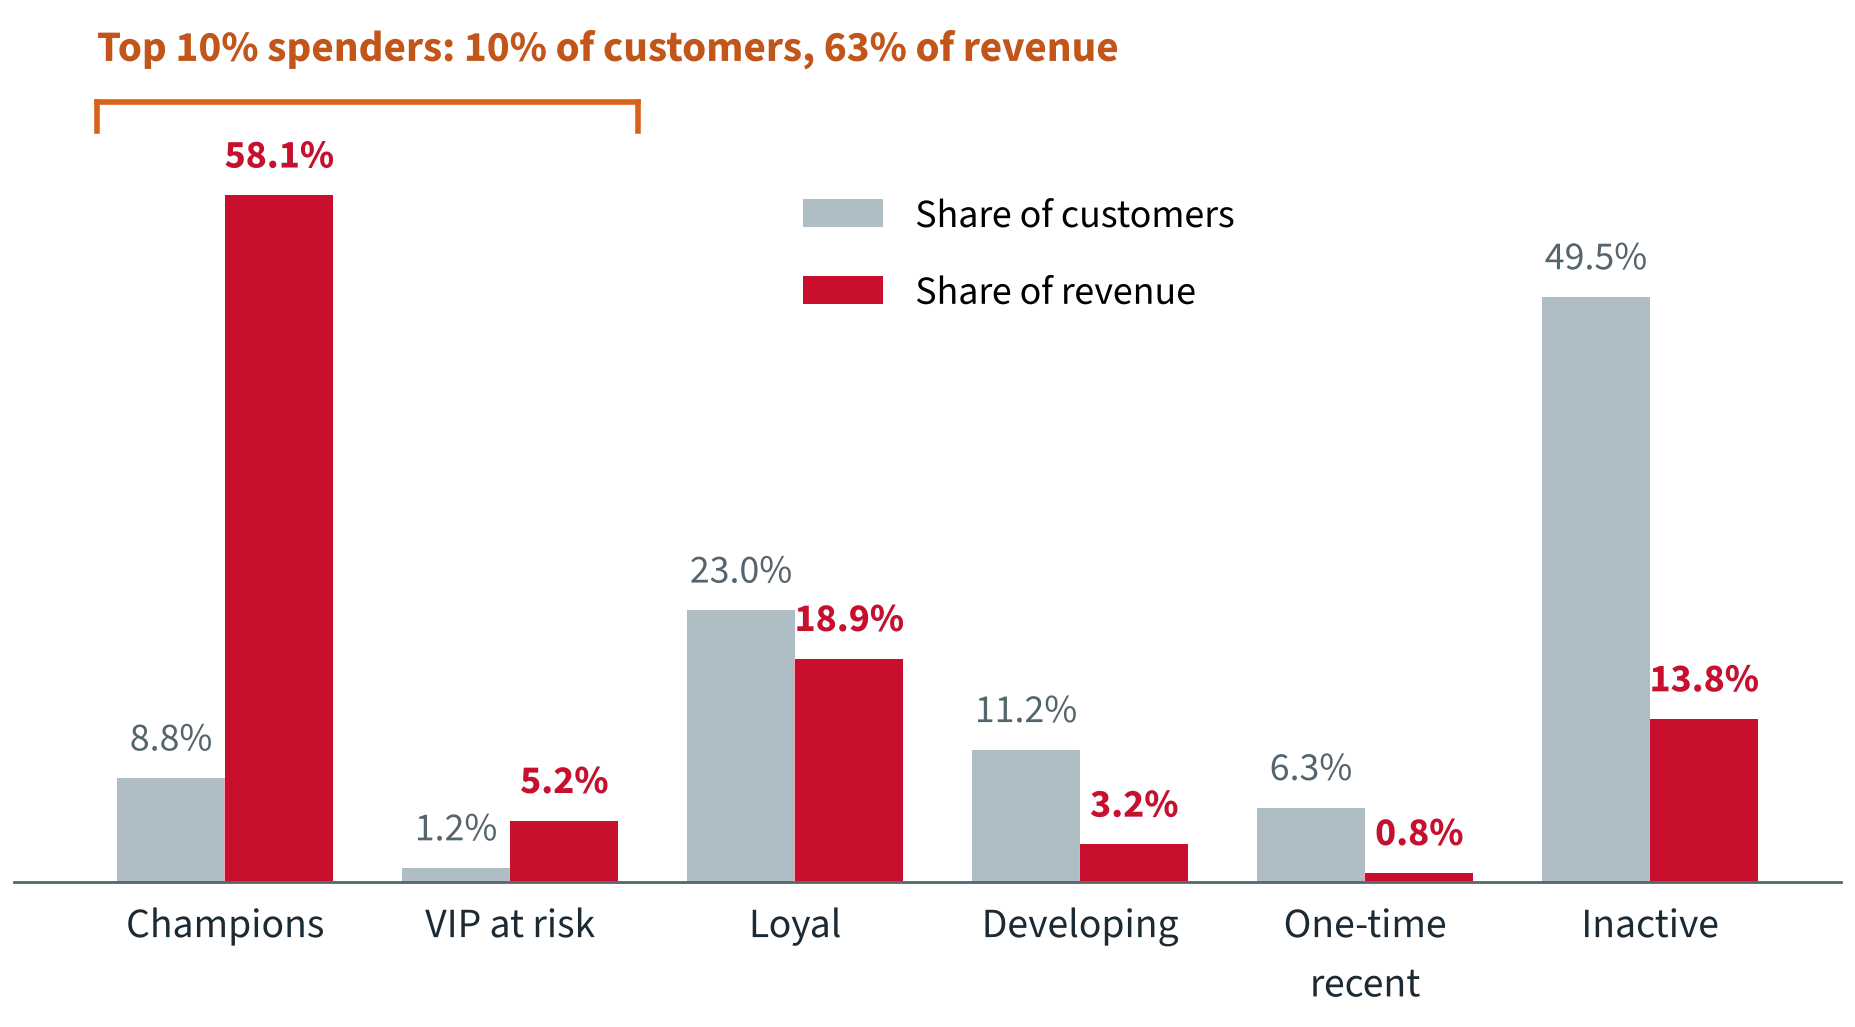
\includegraphics[width=\linewidth]{figures/rfm_segment_share.png}
  \end{columns}
  % Speaker notes (Lam): With that 90-day line and a spend threshold at the top 10\%, we
  % built our RFM segments: recency tells us who is still active, frequency how habitual
  % they are, and spend how valuable they are. The result is very concentrated: Champions
  % and VIP at risk are only 10\% of customers but bring 63\% of revenue. VIP at risk are
  % exactly the high-value customers who have crossed the 90-day line. Meanwhile half of all
  % customers are already inactive and bring only 14\%. So the next step is to predict which
  % valuable customers are about to cross that line, before they do. (About 35 seconds)
\end{frame}

% Churn prediction model (~1 minute, 4 frames). Figures: report Chapters 5-6.
\section{Churn Prediction Model}

% ---- Step card for the preparation pipeline: fixed size, top-aligned ----
\newcommand{\prepstep}[4]{%
  \begin{tikzpicture}[baseline=(card.north)]
    \node (card) [rounded corners=6pt, fill=cardgray, inner sep=8pt] {%
      \parbox[t][3.7cm][t]{2.7cm}{\raggedright
        \cardbadge{#1}\\[6pt]
        {\bfseries\small\color{hustcrimson} #2}\\[2pt]
        {\bfseries\LARGE #3}\\[4pt]
        {\footnotesize\color{inkgray} #4\par}}%
    };
  \end{tikzpicture}%
}
\newcommand{\steparrow}{\raisebox{-2.2cm}{\color{hustcrimson}\Large$\rightarrow$}}

\begin{frame}{Data preparation}{One row per customer per Monday, built only from information up to that date}
  \vspace{0.4cm}
  \centering
  \prepstep{1}{Clean}{72.8\%}{of raw rows kept}%
  \hfill\steparrow\hfill
  \prepstep{2}{Weekly population}{$\sim$2.6k}{active customers per week}%
  \hfill\steparrow\hfill
  \prepstep{3}{Label}{48.0\%}{churn: no purchase in the next 90 days}%
  \hfill\steparrow\hfill
  \prepstep{4}{Features}{11}{RFM\\ Order value\\ Purchase timing\\ Products\\ Cancellations}

  \vspace{0.5cm}
  {\scriptsize\color{inkgray} Active $=$ bought before and last purchase $\leq$ 136 days ago (P90 repurchase gap).}
\end{frame}

\begin{frame}{Data split}{Chronological periods, with a 90-day embargo so no label window reaches the next period}
  \centering
  \includegraphics[width=0.92\textwidth]{figures/split_timeline.png}

  \vspace{0.2cm}
  \small
  \begin{tabular}{@{}llrrr@{}}
    \toprule
    Period & Snapshot dates & Weeks & Rows & Churn rate \\
    \midrule
    Train & Jun -- Nov 2010 & 24 & 61,415 & 43.0\% \\
    Validation & Feb -- Apr 2011 & 8 & 21,514 & 52.9\% \\
    Test & Jul -- Sep 2011 & 10 & 24,252 & 40.1\% \\
    \bottomrule
  \end{tabular}

  \vspace{0.15cm}
  {\scriptsize\color{inkgray} A 6-month warm-up precedes the first snapshot so every customer has some history. The churn rate moves with the season between periods.}
\end{frame}

\begin{frame}{Model experiment}{Final: Logistic Regression $\cdot$ Extended features (8) $\cdot$ $C = 0.01$ $\cdot$ refit on train $+$ validation}
  \begin{columns}[T]
    \column{.63\textwidth}
    \small
    \renewcommand{\arraystretch}{1.08}
    \begin{tabular}[t]{@{}llccc@{}}
      \toprule
      \textbf{Step} & \textbf{Candidate} & \textbf{AUC} & \textbf{Brier} & \\
      \midrule
      Baselines & Random & 0.495 & -- & \\
       & Recency rule & 0.673 & -- & \\
      Training rows & A -- Episode sample & 0.774 & 0.226 & \\
       & B -- All weekly, weighted $1/n_i$ & \textbf{0.781} & \textbf{0.214} & \checkmark \\
      Features & RFM (3) & 0.778 & 0.218 & \\
       & Extended (8) & \textbf{0.781} & \textbf{0.214} & \checkmark \\
       & Full (11) & 0.781 & 0.214 & \\
      Algorithm & Logistic Regression & \textbf{0.781} & \textbf{0.214} & \checkmark \\
       & Random Forest & 0.770 & 0.222 & \\
       & XGBoost & 0.756 & 0.238 & \\
      \bottomrule
    \end{tabular}
    \column{.35\textwidth}
    \small
    \renewcommand{\arraystretch}{1.08}
    \begin{tabular}[t]{@{}lccl@{}}
      \toprule
      \textbf{$C$ (L2)} & \textbf{AUC} & \textbf{Brier} & \textbf{Tied?} \\
      \midrule
      0.001 & 0.775 & 0.213 & no \\
      0.003 & 0.777 & 0.210 & no \\
      \textbf{0.01} & \textbf{0.780} & \textbf{0.210} & \checkmark \\
      0.1 & 0.781 & 0.213 & yes \\
      100 & 0.781 & 0.214 & best \\
      \bottomrule
    \end{tabular}
  \end{columns}
\end{frame}

\begin{frame}{Model evaluation}{Scored once on the 10 test weeks with calibrated probabilities}
  \centering
  \stattile{0.744--0.773}{AUC per week}\hfill
  \stattile{0.194}{Brier score}\hfill
  \stattile{0.110}{HHI of 10 risk bands}\hfill
  \stattile{0.08 $\rightarrow$ 0.14}{CSI vs.\ validation}

  \vspace{0.25cm}
  \begin{columns}[t]
    \column{.49\textwidth}
    \centering
    \includegraphics[width=\textwidth, height=4.4cm, keepaspectratio]{figures/gain_by_decile.png}
    \column{.49\textwidth}
    \centering
    \includegraphics[width=\textwidth, height=4.4cm, keepaspectratio]{figures/shap_summary.png}
  \end{columns}
\end{frame}

% Business impact at an equal discount budget. Numbers: notebooks/06_business_impact.ipynb.
\section{Business Impact}

\begin{frame}{Business impact}{Churn-risk ranking adds the most net margin at equal discount spend (10 held-out weeks, Jul--Sep 2011)}
  \vspace{0.3cm}
  \centering
  \renewcommand{\arraystretch}{1.3}
  \begin{tabular}{@{}lrrr@{}}
    \toprule
    \textbf{How customers are selected} & \textbf{\shortstack[r]{Expected discount\\spend}} & \textbf{Contacts} & \textbf{\shortstack[r]{Simulated increase\\in net margin}} \\
    \midrule
    \textbf{Highest risk of no purchase} & \pounds8,213 & 826 & \textbf{\pounds9,060} \\
    Highest expected margin per contact & \pounds8,219 & 485 & \pounds8,228 \\
    Longest since last purchase & \pounds8,210 & 684 & \pounds6,079 \\
    \bottomrule
  \end{tabular}

  \vspace{0.8cm}
  \raggedright
  {\large Risk ranking adds \textcolor{hustred}{\textbf{\pounds2,982 (49\%)}} in simulated margin over the longest-inactive rule and leads in all ten test weeks under the stated assumptions.\par}
  \vspace{2pt}
  {\small\color{inkgray}Each cohort has a 90-day outcome window. Margin is relative to no offer.\par}
\end{frame}

\begin{frame}{Simulation method}{How the simulation turns offers into incremental profit}
  \vspace{0.2cm}
  \begin{block}{For each customer on the list}
    Expected profit = gross profit on purchases recovered by the offer $-$ discounts on all redeemed orders $-$ contact cost.
  \end{block}
  \vspace{0.3cm}
  \begin{columns}[T]
    \column{.48\textwidth}
    {\large\bfseries Base-case assumptions\par}
    \vspace{6pt}
    {10\% discount, 40\% gross margin and \pounds0.50 per contact.\par}
    \vspace{6pt}
    {The offer recovers 30\% of would-be churners. Among customers who would buy anyway, 40\% redeem it.\par}
    \column{.48\textwidth}
    {\large\bfseries From customer scores to the table\par}
    \vspace{6pt}
    {Add expected profit over the selected customers each week and average across the 10 test weeks.\par}
    \vspace{6pt}
    {For the highest-risk list, \pounds9,060 divided by \pounds8,213 gives \textbf{\pounds1.10 per \pounds1 of discount}.\par}
  \end{columns}
\end{frame}

% Recommendation: weekly policy and the pilot that decides whether to scale.
\section{Recommendation}

\begin{frame}{Recommended next step}{A randomised pilot will tell us whether to scale}
  \vspace{0.2cm}
  \begin{block}{Weekly policy}
    Rank eligible customers by predicted churn risk. Test a 10\% offer under the \pounds8.2K weekly expected discount cap. The simulation shortlisted about 826 customers per week.
  \end{block}
  \vspace{0.3cm}
  \begin{columns}[T]
    \column{.48\textwidth}
    {\large\bfseries Run the pilot\par}
    \vspace{6pt}
    {Recruit 6--8 weekly cohorts. Assign 80\% to receive the offer and 20\% to a no-offer control. Keep assignments fixed and follow each customer for 90 days.\par}
    \column{.48\textwidth}
    {\large\bfseries Decide whether to roll out\par}
    \vspace{6pt}
    {Compare net contribution after discounts, returns and contact costs. Scale if the gain over control is credible and spend stays within the cap. Report one-time and repeat buyers separately.\par}
  \end{columns}
\end{frame}


\begin{hustdarkframe}
  \centering
  \vspace*{0.22\paperheight}
  {\Huge\bfseries\color{white} Thank you!\par}
  \vspace{1.2em}
  {\Large\color{white!85} Questions?\par}
\end{hustdarkframe}

\end{document}
